\documentclass[a4paper]{article}
\usepackage[left=2.1cm, right=2.1cm, top=2.1cm]{geometry}
\usepackage{lipsum}
\usepackage{tikzpagenodes}
\usepackage{pgfplots}
\usepackage{tikz}
\usepackage{tikz-3dplot}
\usetikzlibrary{arrows,decorations.pathmorphing,backgrounds,positioning,fit,matrix}
\pgfplotsset{compat=1.8}
\usepackage{graphics} % for pdf, bitmapped graphics files
\usepackage{epsfig} % for postscript graphics files
\usepackage[colorlinks=true,citecolor=green]{hyperref}
\usepackage{cite}
\usepackage{amsmath,amssymb,amsfonts}
\usepackage{algorithmic}
\usepackage{graphicx}
\usepackage{url}
\usepackage{cite}
\usepackage{bm}
\usepackage{pbox}
\usepackage{siunitx,booktabs,etoolbox}
\usepackage{ulem}
\usepackage[framed,numbered,autolinebreaks,useliterate]{mcode}
\usepackage{filecontents}
%\usepackage{bigfoot} % to allow verbatim in footnote


\def\BibTeX{{\rm B\kern-.05em{\sc i\kern-.025em b}\kern-.08em
    T\kern-.1667em\lower.7ex\hbox{E}\kern-.125emX}}


\begin{document}

\title{Exercise on Multiple Images Stiching}
\author{xiahaa@space.dtu.dk}
\maketitle%%

In this exercise, you will work on using all algorithms you have developed yet to do the stiching for more than two images.

\section{Key Steps}
In order to stich more images, you will have several options:
\subsection{Option $1$}
\begin{enumerate}
\item Choose two images and stich them.
\item Use the stiched image and a third image, stich again.
\item Iterate the previous two steps until all images have been added.
\end{enumerate}
The advantage of this option is easy to implement. However, the disadvantage is the complexity will grow significantly when more images have been stiched because you will have one image quite large.

\subsection{Option $2$}


\begin{figure*}[!b]
	\centering
	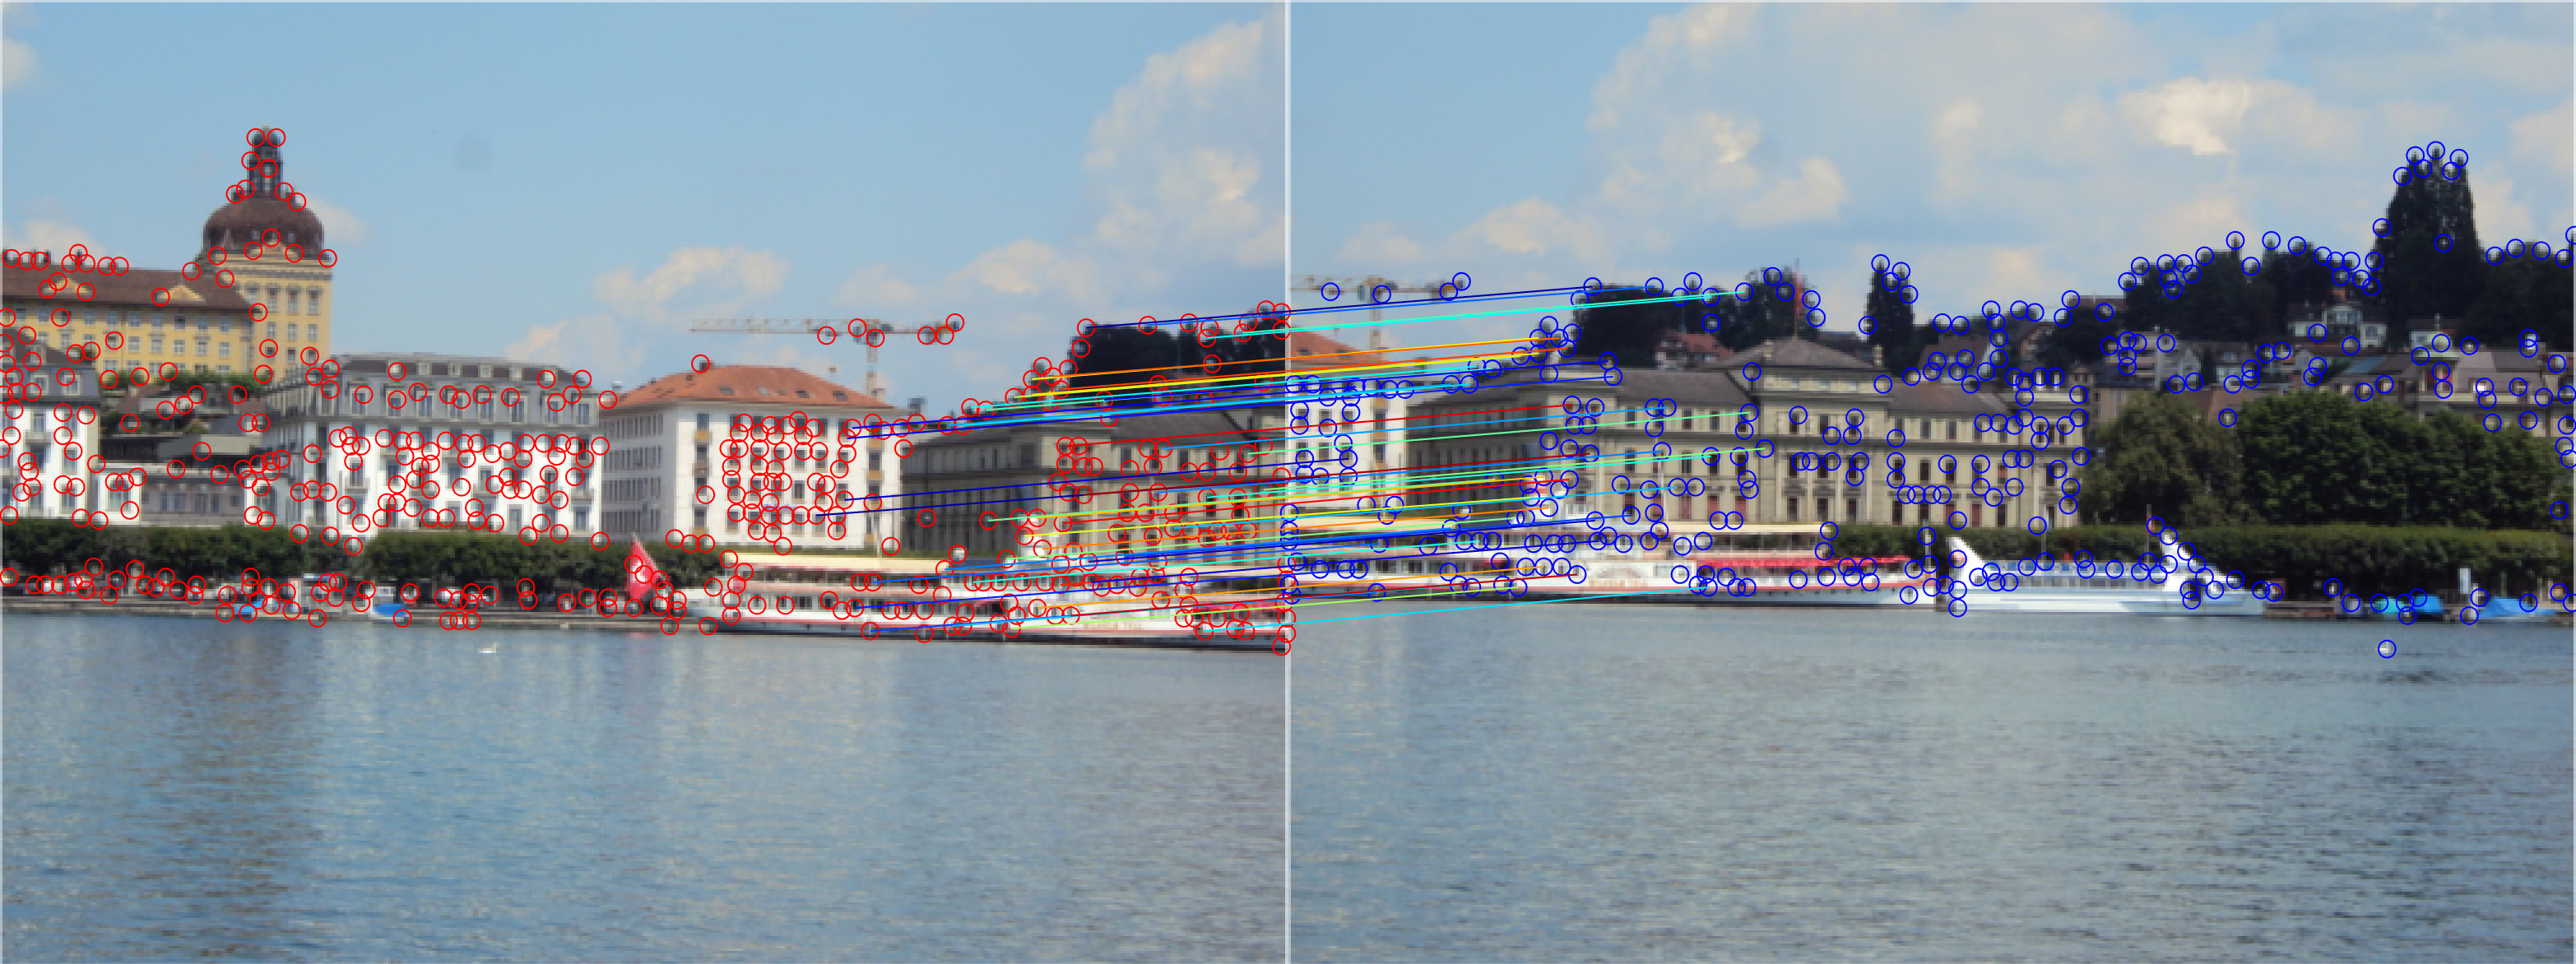
\includegraphics[scale=0.5]{figures/inlier_matches.png}
	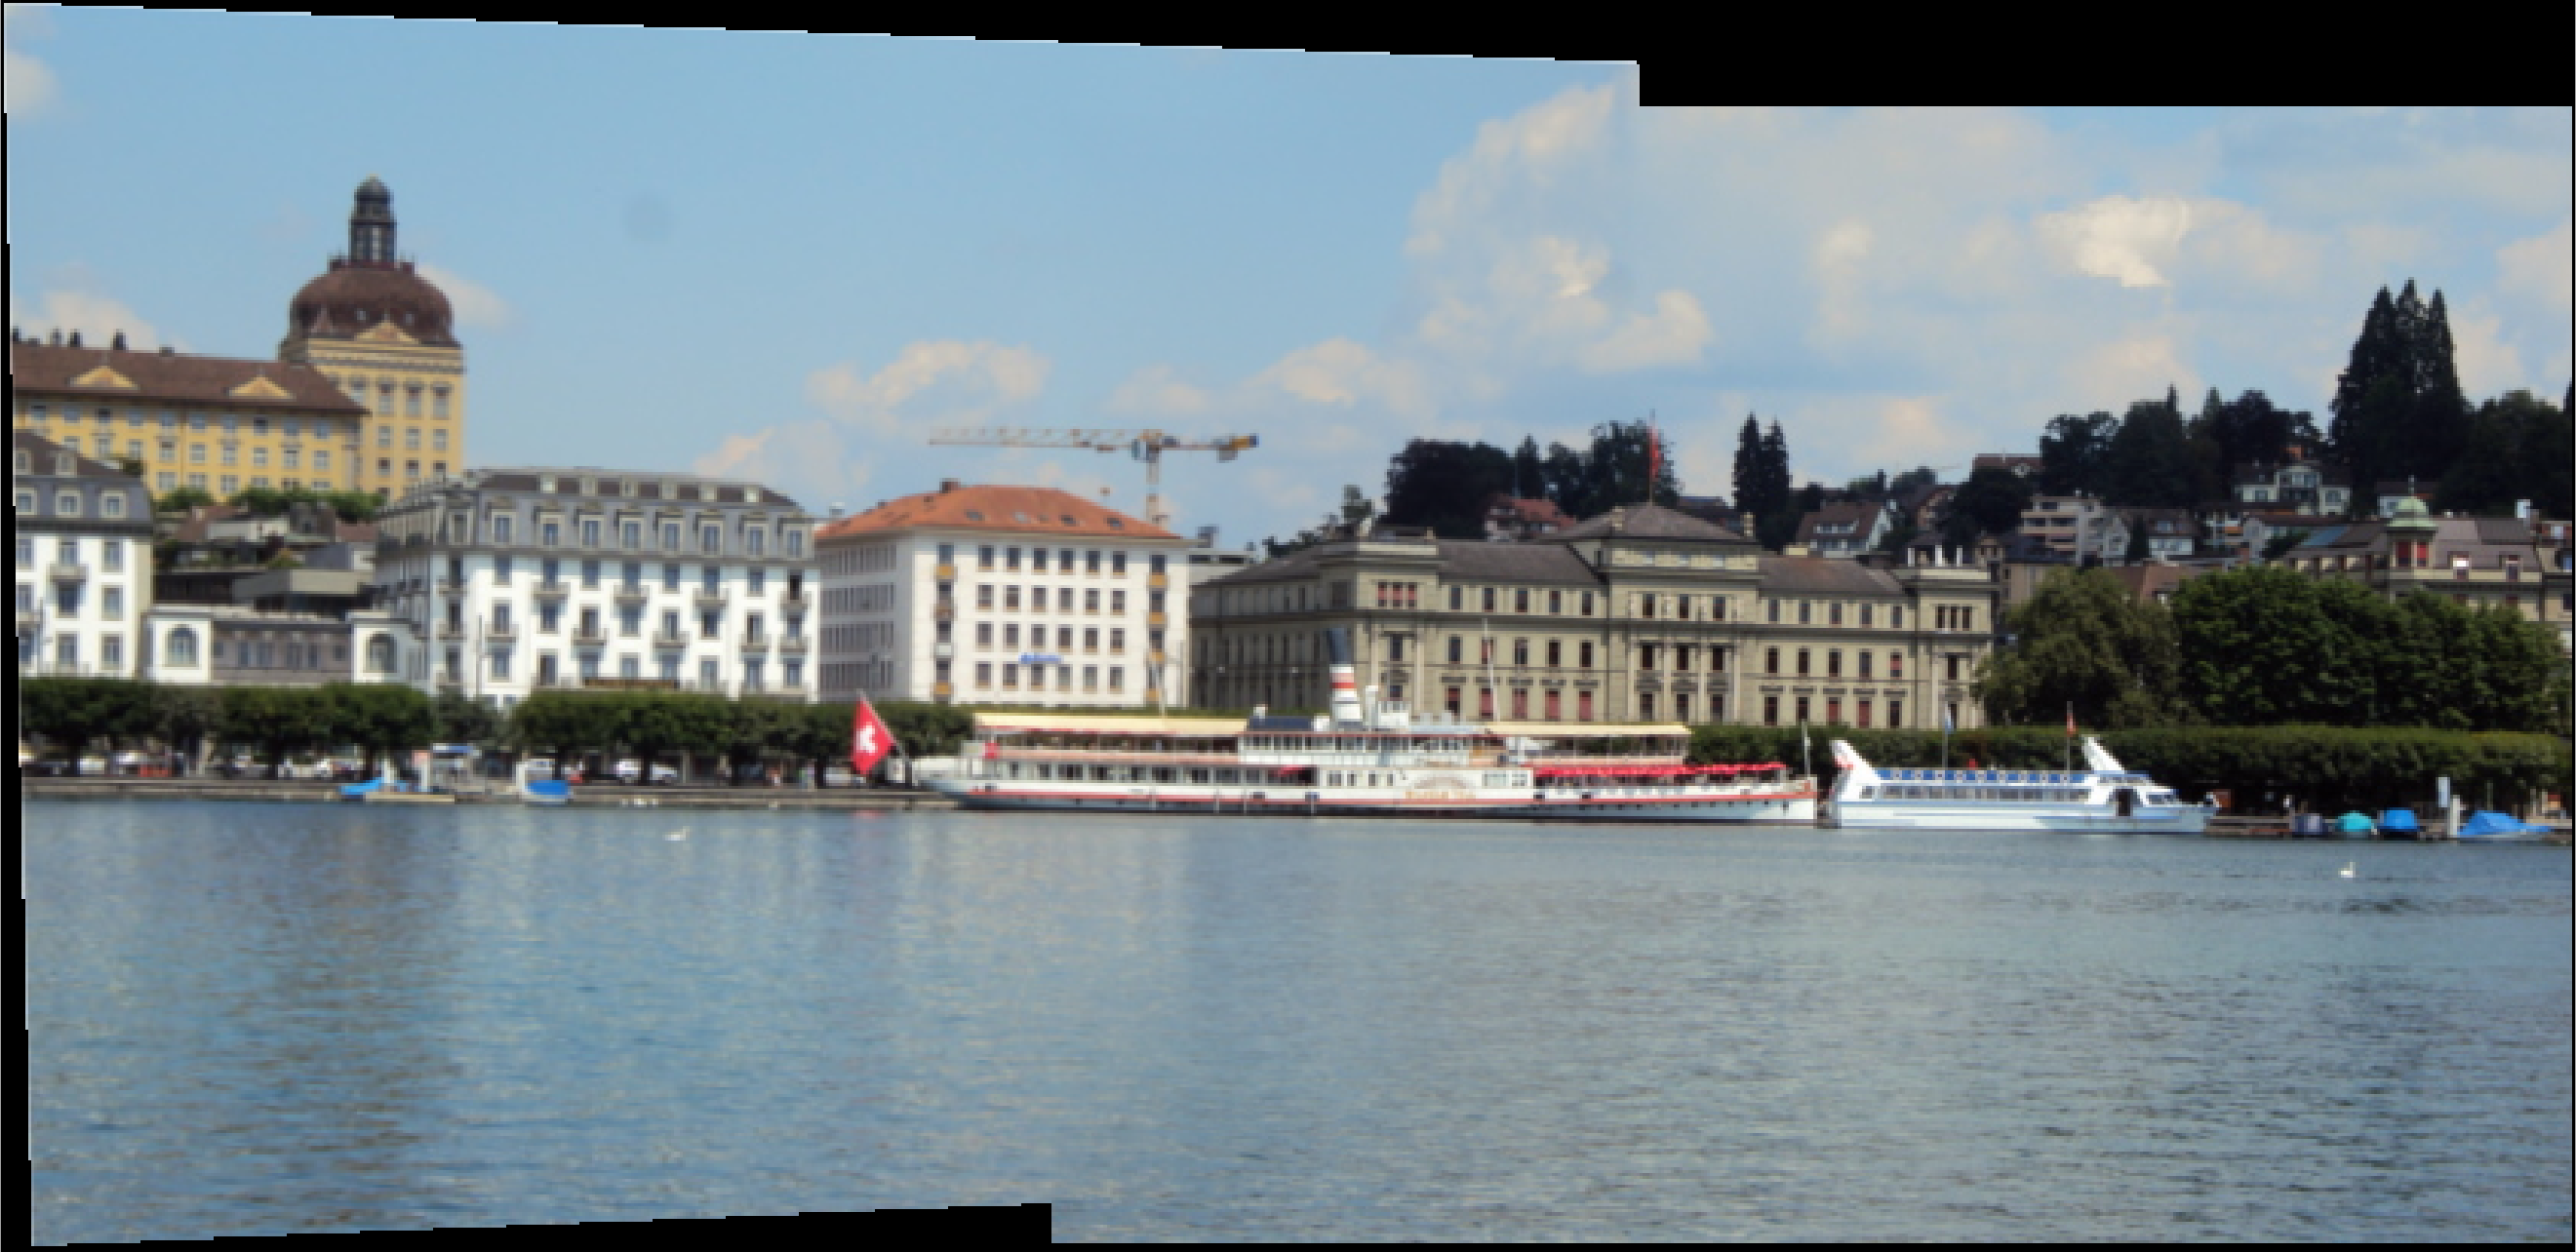
\includegraphics[scale=0.5]{figures/stcih_blend.png}
	\caption{Example of image stich result.}
\end{figure*}

\end{document}